\documentclass{ctexbeamer}        % 文档类beamer的汉化版本

\usefonttheme{serif}              % 使用衬线字体
\usefonttheme{professionalfonts}  % 数学公式字体
\usepackage{amsmath}
\usepackage{mathtools}
\usepackage{hyperref}
\usepackage{listings}
\usepackage{fontspec} % 定制字体
\usepackage{xcolor} % 定制颜色
\usepackage{hyperref}
\definecolor{mygreen}{rgb}{0,0.6,0}
\definecolor{mygray}{rgb}{0.5,0.5,0.5}
\definecolor{mymauve}{rgb}{0.58,0,0.82}
\lstset{ %
backgroundcolor=\color{white},      % choose the background color
basicstyle=\footnotesize\ttfamily,  % size of fonts used for the code
columns=fullflexible,
tabsize=4,
breaklines=true,               % automatic line breaking only at whitespace
captionpos=b,                  % sets the caption-position to bottom
commentstyle=\color{mygreen},  % comment style
escapeinside={\%*}{*)},        % if you want to add LaTeX within your code
keywordstyle=\color{blue},     % keyword style
stringstyle=\color{mymauve}\ttfamily,  % string literal style
frame=none,
rulesepcolor=\color{red!20!green!20!blue!20},
% identifierstyle=\color{red},
language=c++,
}

%% --> 主题和色彩风格
\usetheme{Frankfurt}       %主题和色彩可以自由搭配
\usecolortheme{orchid}     %主题和色彩的样式可参见网页 https://mpetroff.net/files/beamer-theme-matrix/

\newcommand{\qbinom}[2]{\genfrac{[}{]}{0pt}{}{#1}{#2}}
\newcommand{\stirling}[2]{\genfrac\{ \} {0pt}{}{#1}{#2}}
\newcommand{\lcm}{\operatorname{lcm}}
\newcommand{\ord}{\operatorname{ord}}


\begin{document}

%% --> 导言页
%
\title{同余}
\author{Quack}
\date{\today}
\frame{\titlepage}

%% --> 目录结构
\begin{frame}{目录}         %自动生成目录
  \tableofcontents[hideallsubsections]
\end{frame}

%% --> 正式内容开始
\section{定义}

\begin{frame}{定义}

\begin{definition}[同余]
    若$a \bmod p = b \bmod p$,则称$a$和$b$关于(模)$p$同余。记作$a \equiv b \pmod p$。
\end{definition}

\begin{example}
    $5$和$104$关于$3$同余。
\end{example}

本质上,同余关系就是给(非负)整数划分等价类的方式。设我们是在关于$p$同余意义下作讨论,再设两个数$u,v$,若$u \equiv v \pmod p$,那么$u$和$v$是在同一个等价类中;否则$u$和$v$在不同的等价类中。显然一共有$p$个等价类,那么对无限多的(非负)整数的研究就可以转变为对有限的$p$个等价类的研究。

\end{frame}

\AtBeginSection[]{\frame{\tableofcontents[currentsection,hideallsubsections]}}

\section{同余式的运算}

\begin{frame}{同余式的运算}
\begin{theorem}[加乘运算]
    \begin{itemize}
		\item 若$a \equiv b \pmod p$,$c \equiv d \pmod p$,则$a+c \equiv b+d \pmod p$。
		\item 若$a \equiv b \pmod p$,$c \equiv d \pmod p$,则$ac \equiv bd \pmod p$。
		\item 若$a \equiv b \pmod p$,那么对任意整系数多项式$f(x)=a_kx^k+\cdots+a_1x+a_0$,有$f(a) \equiv f(b) \pmod p$。
	\end{itemize}
\end{theorem}
\begin{proof}
    证明的思路是设$a=k_ap+r$,然后去推就可以了。
\end{proof}
这几条定理说明了同余式的两端可以同时加(减)乘一个相同的数(或两个同余的数)。
\end{frame}

\begin{frame}{同余式的运算}
\begin{theorem}[更换模数]
    \begin{itemize}
		\item 若$a \equiv b \pmod m$,$d|m$,则$a \equiv b \pmod d$。
		\item 若$ac \equiv bc \pmod m$,则$a \equiv b \pmod {\frac{m}{\gcd(c,m)}}$。
	\end{itemize}
\end{theorem}
\begin{proof}
	\begin{itemize}
    	\item $a \equiv b \pmod m$,即$m|(a-b)$,又有$d|m$,则$d|(a-b)$,所以$a \equiv b \pmod d$。
    	\item $ac \equiv bc \pmod m$,即$m|(ac-bc)$,则$\frac{m}{\gcd(c,m)}|(a-b)$,所以$a \equiv b \pmod {\frac{m}{\gcd(c,m)}}$。
    \end{itemize}
\end{proof}
第一条定理说明了研究模合数的同余可以转化为研究模素数幂的同余。例如,$a \equiv b \pmod{12}$等价于$a \equiv b \pmod 4$且$a \equiv b \pmod 3$。

第二条定理说明了同余式的两端不能直接除以一个相同的数。
\end{frame}

\section{剩余系}
\begin{frame}{剩余系}

\begin{definition}[剩余系]
    模$m$的剩余系是一个集合,由模$m$两两不等的$m$个数组成。

	把$\lbrace 0,1,\cdots,m-1 \rbrace$称为模$m$的标准剩余系。
\end{definition}

本质上,模$m$意义下的同余关系将(非负)整数划分成了$m$个等价类,模$m$的剩余系就是在这$m$个等价类中,每个等价类挑了一个元素出来作为这个等价类的代表元。剩余系主要是辅助证明一些数论定理的工具。

\end{frame}

\begin{frame}{剩余系}

\begin{theorem}[构造剩余系]
    若$S=\lbrace a_1,\cdots,a_m \rbrace$是模$m$的一个剩余系,那么$S'=\lbrace ka_1+b,\cdots,ka_m+b \rbrace$也是模$m$的一个剩余系,其中$\gcd(k,m)=1$。
\end{theorem}

\begin{proof}
	由剩余系的定义,显然$|S'|$在大小上是符合条件的。只需证$S'$内元素模$m$两两不等即可。

	即考虑证明当$i \neq j$时,$ka_i+b \neq ka_j+b \pmod m$。用反证法容易证出。
\end{proof}

\end{frame}

\begin{frame}{剩余系}

\begin{definition}[缩系]
    模$m$的缩系(简化剩余系、既约剩余系)是一个集合,由模$m$两两不等且与$m$互质的若干个数组成。
\end{definition}

\begin{definition}[欧拉函数]
    设$0$到$m-1$的整数中,有$\varphi(m)$个数和$m$互质,把$\varphi(m)$叫做欧拉函数。显然模$m$的缩系大小为$\varphi(m)$。
\end{definition}

\begin{example}
    $\lbrace 1,3,7,9 \rbrace$是$10$的缩系。

	$\varphi(10)=4$。
\end{example}

\end{frame}

\begin{frame}{剩余系}

\begin{theorem}[构造缩系]
    若$S=\lbrace a_1,\cdots,a_t \rbrace$是模$m$的一个缩系,那么$S'=\lbrace ka_1,\cdots,ka_t \rbrace$也是模$m$的一个剩余系,其中$\gcd(k,m)=1$。
\end{theorem}

\begin{proof}
	由缩系的定义,显然$|S'|$在大小上是符合条件的。只需证$S'$内元素模$m$两两不等且都和$m$互质即可。

	即考虑证明当$i \neq j$时,$ka_i \neq ka_j \pmod m$且$\gcd(ka_i,m)=1$。用反证法容易证出。
\end{proof}

\end{frame}

\begin{frame}{剩余系}

\begin{theorem}[欧拉定理]
    若$\gcd(a,m)=1$,则$a^{\varphi(m)}\equiv 1 \pmod m$。
\end{theorem}
\pause
\begin{proof}
	设$S=\lbrace c_1,\cdots,c_t \rbrace$是模$m$的一个缩系。

	由于$\gcd(a,m)=1$,$S'=\lbrace ac_1,\cdots,ac_t \rbrace$也是模$m$的一个缩系。

	显然,两个缩系的积在模$m$意义下相等,即$\prod_{i=1}^t c_i \equiv a^t \prod_{i=1}^t c_i \pmod m$。

	又因为缩系里任意一个元素都和$m$互质,可以左右消去,所以有$a^t \equiv 1 \pmod m$,其中,$t$为缩系的大小,显然是$\varphi(m)$。
\end{proof}

欧拉定理的一个常见用法是对指数降幂。

\end{frame}

\begin{frame}{剩余系}

\begin{theorem}[费马小定理]
    若$p$为质数,则对任意的$a$,有$a^p\equiv a \pmod p$。
\end{theorem}
\pause
\begin{proof}
	分类讨论:若$p|a$,则左右都是$0$,显然成立;否则有$\gcd(a,p)=1$,由欧拉定理易得。
\end{proof}

费马小定理的一个常见用法是,若对给定的$p$和任意的$a$,都使得$a^p\equiv a \pmod p$,则说明$p$有可能是一个质数。

然后就引出有错误概率的质数判定算法。这里不作展开。

\end{frame}

\begin{frame}{剩余系}

\begin{theorem}[威尔逊定理]
    $(p-1)!\equiv -1 \pmod p$当且仅当$p$为质数。
\end{theorem}
\pause
\begin{proof}
	从$p$为质数导出$(p-1)! \equiv -1 \pmod p$:
	
	由费马小定理可得,当$p$为质数的时候,$x=1,2,3,\cdots,p-1$都是方程$x^{p-1}\equiv 1 \pmod p$的解。所以有

	$$x^{p-1}-1 \equiv (x-1)(x-2)\cdots (x-(p-1)) \equiv 0 \pmod p$$

	取$x=p$即得威尔逊定理。

	从$(p-1)!\equiv -1 \pmod p$导出$p$为质数:

	反证法,若$p$不是质数,则存在一个小于$p$的质数$q$,使得$q|p$。

	那么$(p-1)! \equiv 0 \pmod q$,和$(p-1)! \equiv -1 \pmod p$矛盾。
\end{proof}

\end{frame}

\begin{frame}{剩余系}

\begin{theorem}[欧拉函数的积性]
    若$\gcd(a,b)=1$,则$\varphi(ab)=\varphi(a)\varphi(b)$。
\end{theorem}

\begin{proof}
	设$S_a=\lbrace x_1,x_2,\cdots,x_{\varphi(a)} \rbrace$和$S_b=\lbrace y_1,y_2,\cdots,y_{\varphi(b)} \rbrace$分别是模$a$和模$b$的一个缩系。

	我们构造模$ab$的缩系$S_{ab}=\lbrace bx_i+ay_j|1\le i\le \varphi(a),1\le j\le \varphi(b) \rbrace$。

	由缩系性质易知,如果$x_i \neq x_{i'}$或者$y_j \neq y_{j'}$,那么$bx_i+ay_j \neq bx_{i'}+ay_{j'}$。因此$S_{ab}$中元素两两不等,即$|S_{ab}|=\varphi(a)\varphi(b)$。只要我们证明了$S_{ab}$确实是模$ab$的缩系,我们就证明了$\varphi(ab)=\varphi(a)\varphi(b)$。
\end{proof}

\end{frame}

\begin{frame}{剩余系}

\begin{theorem}[欧拉函数的积性]
    若$\gcd(a,b)=1$,则$\varphi(ab)=\varphi(a)\varphi(b)$。
\end{theorem}

\begin{proof}
	证明缩系$S_{ab}$是模$ab$的缩系分为两步:
	\begin{itemize}
		\item 元素两两不等,已经(简单地)证过了;
		\item 对任意的$i,j$,有$\gcd(bx_i+ay_j,ab)=1$。要证这个,我们只需证$\gcd(bx_i+ay_j,a)=1$且$\gcd(bx_i+ay_j,b)=1$,显然都是很好证明的。
	\end{itemize}
\end{proof}

\end{frame}

\begin{frame}{剩余系}

\begin{theorem}[欧拉函数计算公式]
    \begin{itemize}
		\item 若$p$是质数且$\alpha \ge 1$,则$\varphi(p^{\alpha})=p^{\alpha} - p^{\alpha-1}$。
		\item 设$m$的标准分解为$m=p_1^{\alpha_1}p_2^{\alpha_2}\cdots p_k^{\alpha_k}$,则$$\varphi(m)=m(1-\frac{1}{p_1})(1-\frac{1}{p_2})\cdots(1-\frac{1}{p_k})$$
	\end{itemize}
\end{theorem}

\begin{proof}
	\begin{itemize}
		\item 考虑模$p^{\alpha}$的标准剩余系$S=\lbrace 0,1,2,\cdots,p^{\alpha}-1 \rbrace$,在$S$中与$p^{\alpha}$不互质的数只有$p$的倍数,即$0,p,2p,\cdots,p^{\alpha-1}$。所以和$p^{\alpha}$互质的数就有$p^{\alpha}(1-\frac{1}{p})=p^{\alpha} - p^{\alpha-1}$个。
		\item 由欧拉函数的积性不难证明。
	\end{itemize}
\end{proof}

因此,求单个数的欧拉函数的复杂度和对这个数分解质因数的复杂度相同。

\end{frame}

\begin{frame}{剩余系}

\begin{theorem}[欧拉函数其他性质]
    \begin{itemize}
		\item 设$\gcd(a,b)=d$,那么$\varphi(ab)=\varphi(a)\varphi(b)\frac{d}{\varphi(d)}$。
		\item 若$a|b$,则$\varphi(a)|\varphi(b)$。
	\end{itemize}
\end{theorem}

\begin{proof}
	对于这两个性质,都只需证在质数的幂处的取值满足条件,然后用积性就可以证出来了。在质数的幂处的取值满足条件是容易证的。
\end{proof}

\end{frame}

\begin{frame}{剩余系}

\begin{theorem}[欧拉函数其他性质]
	设$m$是正整数,则$\sum_{d|m} \varphi(d) = m$。
\end{theorem}
\pause
\begin{proof}
	考虑有理数集$S=\lbrace \frac{r}{m} | r=1,2,\cdots,m \rbrace$。设$S'$是将$S$中每个$\frac{r}{m}$约分后所得的集合。由于约分不改变分数的值,$S'$中没有两个分数的值是相等的。反之,对于$\gcd(c,d)=1,c\le d,d|m$的所有分子$\frac{c}{d}$,设$m=kd$,由于$\frac{kc}{m}$在$S$中,所以$\frac{c}{d}$在$S'$中。

	考虑枚举$S'$中的所有分数,一种枚举的方法就是先枚举分母,再枚举分子。由于$S'$中的分数是约分来的,所以枚举的分母$d$满足$d|m$。由于这是既约分数,所以分子要和分母$d$互质。又因为$|S'|=m$,所以$\sum_{d|m} \varphi(d) = m$。
\end{proof}

\end{frame}

\begin{frame}{剩余系}

\begin{theorem}[欧拉函数其他性质]
	小于$m$且与$m$互质的所有正整数之和为$m\frac{\varphi(m)}{2}$。
\end{theorem}
\pause
\begin{proof}
	设$S=\lbrace c_1,\cdots,c_t \rbrace(1 \le c_i < m)$是模$m$的一个缩系。

	$S'=\lbrace m-c_1,\cdots,m-c_t \rbrace$也是模$m$的一个缩系,并且$S'$的每个元素也是在大于$0$小于$m$的范围内的。

	所以两个缩系的和相等,即$\sum_{i=1}^t c_i = m\varphi(m) - \sum_{i=1}^t c_i$。

	所以小于$m$且与$m$互质的所有正整数之和为$m\frac{\varphi(m)}{2}$。
\end{proof}

\end{frame}

\section{练习}

\begin{frame}{练习}{欧拉定理}

\begin{example}[欧拉降幂]
	求$a^{\text{一个很大的数,如高精度数}} \bmod m$,其中$\gcd(a,m)=1$。
\end{example}
\pause
设这个很大的数为$C$,那么由欧拉定理我们有$a^C \equiv a^{C \bmod \varphi(m)} \pmod m$。

然后需要算高精度数模低精度数,还有就是快速幂。

\end{frame}

\begin{frame}{练习}{欧拉定理}

\begin{example}[accoders 9952]
	给定一个质数$p$,有递推数列$E$,满足$E_1=E_2=p,E_i=E_{i-1}E_{i-2}$。再给定一个数$q$,满足$0<q<p$,求$E_n \bmod q$。

	数据范围:多组数据,$T\le 5000$,$0<p,n<2^{31}$。
\end{example}
\pause
可以写出$E_n$的通项:$E_n=p^{f_n}$,其中,$f_n$是fib数列的第$n$项($f_1=f_2=1$)。由欧拉降幂,$E_n \bmod q \equiv p^{f_n \bmod \varphi(q)} \pmod q$。

$f_n \bmod \varphi(q)$可以用矩阵快速幂来计算。然后再来个快速幂即可计算出$p^{f_n \bmod \varphi(q)}$。

\end{frame}

\begin{frame}{练习}{欧拉定理}

\begin{example}[accoders 6095]
	给定$a,b,c,d,n,m$,有递推数列$F$,满足$F(i,j)=aF(i,j-1)+b(j>1)$且$F(i,1)=cF(i-1,m)+d$。递推数列的初值为$F(1,1)=1$。

	求$F(n,m) \bmod 10^9+7$。

	数据范围:$1\le n,m \le 10^{1000000}$,$1\le a,b,c,d \le 10^9$。
\end{example}
\pause
不难写出当行转移矩阵$A=\begin{pmatrix} a & b \\ 0 & 1 \end{pmatrix}$和换行转移矩阵$B=\begin{pmatrix} c & d \\ 0 & 1 \end{pmatrix}$。那么有
$$A^{m-1}(BA^{m-1})^{n-1}\begin{pmatrix} F(1,1) \\ 1 \end{pmatrix} = \begin{pmatrix} F(n,m) \\ 1 \end{pmatrix}$$
直接矩阵快速幂可能因为常数过大而超时。

\end{frame}

\begin{frame}{练习}{欧拉定理}

设$p=10^9+7$,我们考虑能否搞一个矩阵的欧拉定理,下面均在模$p$意义下推导:
$$\begin{pmatrix} a & b \\ 0 & 1 \end{pmatrix}^{p-1}=\begin{pmatrix} a^{p-1} & b(1+a+\cdots+a^{p-2}) \\ 0 & 1 \end{pmatrix}=\begin{pmatrix} 1 & 0 \\ 0 & 1 \end{pmatrix}$$
并且我们还发现$\begin{pmatrix} a & b \\ 0 & 1 \end{pmatrix}\begin{pmatrix} c & d \\ 0 & 1 \end{pmatrix}=\begin{pmatrix} ac & ad+b \\ 0 & 1 \end{pmatrix}$,所以在计算$A^{m-1}(BA^{m-1})^{n-1}$时,指数也可以像计算数的幂一样,在指数上模$\varphi(p)$。

注意这只是对形如$\begin{pmatrix} a & b \\ 0 & 1 \end{pmatrix}$这样的矩阵有欧拉定理,对任意的矩阵,欧拉定理不一定成立。
\end{frame}

\begin{frame}{练习}{欧拉定理}

\begin{example}[计算阶]
	设$\gcd(a,m)=1$,把最小的使得$a^c \equiv 1 \pmod m$的正整数$c$记作$\ord_{m}(a)$,即$a$对$m$的阶。

	如何计算$\ord_{m}(a)$?
\end{example}
\pause
由欧拉定理$a^{\varphi(m)}\equiv 1 \pmod m$,所以$\ord_{m}(a)|\varphi(m)$。

注意到由$m$的质因数分解我们可以直接得到$\varphi(m)$的质因数分解,然后从小到大枚举因数验证即可。

\end{frame}

\begin{frame}{练习}{欧拉定理}

\begin{example}[循环小数]
	设既约分数$\frac{a}{b}(0\le a<b,\gcd(a,b)=1)$,求把$\frac{a}{b}$转为小数后,其最小循环节和不循环部分的长度。
\end{example}
\pause
设循环节长为$l$,不循环部分长为$c$,那么有$10^{l+c} \cdot a \equiv 10^c \cdot a \pmod b$,由于$\gcd(a,b)=1$,所以$10^{l+c} \equiv 10^c \pmod b$。

如果$\gcd(10,b) = 1$,那么$10^l \equiv 1 \pmod b$,那么$l=\ord_b(10)$,并且小数没有不循环的部分。

如果$\gcd(10,b) \neq 1$,那么设$b=2^{k_2}5^{k_5}b',\gcd(10,b')=1$,由$10^{l+c} \equiv 10^c \pmod b$可得$10^{l+c} \equiv 10^c \pmod{b'}$,即$10^l \equiv 1 \pmod{b'}$,$l=\ord_{b'}(10)$。显然小数循环的部分是$c=\max(k_2,k_5)$。当然,若$b'=1$,那么小数没有循环节。
\end{frame}

\begin{frame}{练习}{欧拉函数}

\begin{example}[仪仗队]
	给定整数$n$,求$1\le x,y \le n$且$\gcd(x,y)=1$的数对$(x,y)$有多少对。

	数据范围:$n\le 10^7$。
\end{example}
\pause
推一波式子:
$$\sum_{x=1}^n \sum_{y=1}^n [\gcd(x,y)=1]=2\sum_{x=1}^n \sum_{y=1}^{x} [\gcd(x,y)=1] - 1=2\sum_{x=1}^n \varphi(x) - 1$$

相当于要求欧拉函数的前缀和,后面我们会讲一个线性筛的做法。
\end{frame}

\begin{frame}{练习}{欧拉函数}

\begin{example}[仪仗队]
	给定整数$n$,求$1\le x,y \le n$且$\gcd(x,y)=1$的数对$(x,y)$有多少对。

	数据范围:$n\le 10^7$。
\end{example}
这个题叫仪仗队是因为求的这个东西有一个组合意义:
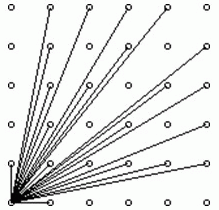
\includegraphics[scale=0.6]{figure1.png}
\end{frame}

\begin{frame}{练习}{欧拉函数}

\begin{example}[accoders2564]
	给定整数$n$,求$1\le x,y \le n$且$\gcd(x,y)$为质数的数对$(x,y)$有多少对。

	数据范围:$n\le 10^7$。
\end{example}
\pause
推一波式子:
$$\sum_{x=1}^n \sum_{y=1}^n [\gcd(x,y)\text{是质数}]=\sum_{p\text{是质数}} \sum_{x=1}^{\frac{n}{p}} \sum_{y=1}^{\frac{n}{p}} [\gcd(x,y)=1]$$
\end{frame}

\begin{frame}{练习}{欧拉函数}

\begin{example}[accoders2564]
	给定整数$n$,求$1\le x,y \le n$且$\gcd(x,y)$为质数的数对$(x,y)$有多少对。

	数据范围:$n\le 10^7$。
\end{example}
推一波式子:
$$\sum_{x=1}^n \sum_{y=1}^n [\gcd(x,y)\text{是质数}]=\sum_{p\text{是质数}}(2\sum_{x=1}^{\frac{n}{p}} \varphi(x) - 1)$$
\end{frame}

\begin{frame}{练习}{欧拉函数}

\begin{example}[accoders6110]
	给定整数$n$,求$\sum_{i=1}^n \gcd(i,n)$。

	数据范围:$n\le 2^{32}$。
\end{example}
\pause
推一波式子:
$$\sum_{i=1}^n \gcd(i,n)=\sum_{d|n} d\varphi(\frac{n}{d})$$

这个式子可以暴力算,也能观察出这个是$\varphi$和$Id$的狄利克雷卷积,那么答案也是一个积性函数,通过求其在质数的幂处的取值,再利用积性即可求出在$n$处的取值。时间复杂度$O(\sqrt{n})$。
\end{frame}

\section{extra}

\begin{frame}{gcd matrix}

\begin{example}
	设$n$阶矩阵$A$,其$i$行$j$列的元素$a_{ij}$满足$a_{ij}=\gcd(i,j)$。

	求$|A|$。
\end{example}
\pause
做矩阵分解,构造矩阵$B$,$C$,使得$A=BC^T$,则$|A|=|B||C|$。

其中,当$j|i$,$b_{ij}=g(j)$,否则$b_{ij}=0$。当$j|i$,$c_{ij}=1$,否则$c_{ij}=0$。

那么,$a_{ij}=\sum_{k=1}^n b_{ik}c_{jk}=\sum_{k|\gcd(i,j)}g(k)$。

由于$\sum_{d|m} \varphi(d) = m$,所以取$g=\varphi$,那么$a_{ij}=\gcd(i,j)$。

所以$|A|=|B||C|=\prod_{i=1}^n \varphi(i)$。
\end{frame}

\begin{frame}{gcd matrix}

\begin{example}
	设$n$阶矩阵$A$,其$i$行$j$列的元素$a_{ij}$满足$a_{ij}=f(\gcd(i,j))$。

	求$|A|$。
\end{example}
设$f(n)=\sum_{d|n} g(d)$,那么由还没讲过的莫比乌斯反演,有$g(n)=\sum_{d|n}u(d)f(\frac{n}{d})$,所以$|A|=\prod_{i=1}^n g(i)$。
\end{frame}

\begin{frame}{gcd matrix}

\begin{example}[poj3910]
	设$n$阶矩阵$A$,其$i$行$j$列的元素$a_{ij}$满足$a_{ij}=\gcd(s_i,s_j)$。

	求$|A|$。其中$S=\lbrace s_1,\cdots,s_n \rbrace$,$S$满足一个条件:若$x \in S$,则对所有的$d|x$,有$d \in S$(这个条件可以换成一个更强的条件:若$x,y \in S$,则$\gcd(x,y) \in S$)。
\end{example}
我们不加证明地给出答案$|A|=\prod_{i=1}^n \varphi(s_i)$。
\end{frame}

\begin{frame}{lucas定理}

\begin{theorem}[lucas]
	对质数$p$,有:
	$$\binom{n}{m} \equiv \binom{n/p}{m/p} \binom{n \bmod p}{m \bmod p} \pmod p$$
\end{theorem}
先证明一个引理:
\begin{theorem}
	对质数$p$,有:
	$$(1+x)^p \equiv 1+x^p \pmod p$$
\end{theorem}
\begin{proof}
	只需证明对任意的$i=2,3,\cdots,p-1$,有$p|\binom{p}{i}$即可。
	
	这是好证的。
\end{proof}
\end{frame}

\begin{frame}{lucas定理}

\begin{theorem}[lucas]
	对质数$p$,有:
	$$\binom{n}{m} \equiv \binom{n/p}{m/p} \binom{n \bmod p}{m \bmod p} \pmod p$$
\end{theorem}
\begin{proof}
	设$n=kp+r$,那么$(1+x)^n \equiv (1+x)^{kp} (1+x)^r \equiv (1+x^p)^k (1+x)^r \pmod p$。

	两边提取$x^m$系数,有$\binom{n}{m} \equiv [x^m](1+x)^n \equiv [x^m](1+x^p)^k (1+x)^r \equiv \binom{n/p}{m/p} \binom{n \bmod p}{m \bmod p} \pmod p$。
\end{proof}
\end{frame}

\begin{frame}[plain]    %%谢谢
	\vspace{0.4\textheight}
	\begin{center}
		\Huge\color{blue}\bfseries Thanks!
	\end{center}
\end{frame}

\end{document}